\documentclass[conference]{IEEEtran}
\IEEEoverridecommandlockouts
% The preceding line is only needed to identify funding in the first footnote. If that is unneeded, please comment it out.
\usepackage{cite}
\usepackage{amsmath,amssymb,amsfonts}
\usepackage{algorithmic}
\usepackage{graphicx}
\usepackage{textcomp}
\usepackage{xcolor}
\usepackage{placeins}
\usepackage{float}
\usepackage{listings}
\def\BibTeX{{\rm B\kern-.05em{\sc i\kern-.025em b}\kern-.08em
    T\kern-.1667em\lower.7ex\hbox{E}\kern-.125emX}}
\begin{document}

\title{Aplicación de Machine Learning en el Conjunto de Datos Iris\\
{\footnotesize \textsuperscript{}Asignación 2}
\thanks{}
}

\author{\IEEEauthorblockN{\textsuperscript{} María José Porras Maroto}
\IEEEauthorblockA{\textit{Tecnológico de Costa Rica, Escuela de Ingeniería en Computación} \\
\textit{Inteligencia Artificial - IC6200 - Grupo 2}\\
Email: marijopm27@estudiantec.cr}
}



\maketitle

\begin{abstract}
This document presents an analysis of the construction and evaluation of a K-Nearest Neighbors (KNN) algorithm, focusing on feature selection and experimentation with various values of K to optimize precision. 
\end{abstract}

\begin{IEEEkeywords}
component, formatting, style, styling, insert
\end{IEEEkeywords}

\section{Introducción}
El presente informe detalla los resultados obtenidos de las diversas evaluaciones realizadas sobre el conjunto de datos iris. La exploración realizada permite no solo valorar las diversas características del dataset, sino que también permite valorar el rendimiento del algoritmo KNN para la categorización de especies de flores. Igualmente, este documento permite al estudiantado comprender en mayor profundidad la elaboración, implementación y evaluación de un modelo de Machine Learning.

\section{Objetivos}
\begin{enumerate}

    \item Realizar una exploración de las características del conjunto de datos Iris, comprendiendo los detalles detras de los features y su distribución.
    
    \item Implementar el algoritmo de k-Nearest Neighbors (KNN) sin la utilización de bibliotecas preexistentes, asegurando una comprensión profunda de su funcionamiento y parámetros.
    
    \item Experimentar con parámetros en el algoritmo KNN para optimizar su rendimiento en la clasificación de las especies de flores Iris.
    
    \item Evaluar el modelo KNN utilizando métricas de precisión, proporcionando una medida cuantitativa de su capacidad para clasificar correctamente las especies de flores Iris.

\end{enumerate}

\section{Análisis del Conjunto de Datos}
Tras la carga del conjunto de datos al notebook, es posible realizar una lectura de los mismos y obtener especificaciones sobre las clasificaciones y características que lo conforman. Algunos de los detalles explorados sobre el conjunto de datos se explica a continuación.

\subsection{Detalles del conjunto de datos}
Mediante la librería de pandas no solo es posible realizar la carga y lectura de los datos, sino que posee diversas funciones para obtener datos asociados al dataset en cuestión. Por medio de las instrucciones .info() es que se logra obtener un resumen sobre el conjunto, incluyendo datos como el número de columnas, número de valores no nulos de cada columna y el tipo de dato de cada columna

\begin{table}[h]
\centering
\caption{Resumen del DataFrame}
\label{tab:resumen_dataframe}
\begin{tabular}{|l|c|c|}
\hline
\textbf{Columna} & \textbf{Valores no Nulos} & \textbf{Tipo de Dato} \\ \hline
sepal\_length & 150 & float64 \\
sepal\_width & 150 & float64 \\
petal\_length & 150 & float64 \\
petal\_width & 150 & float64 \\
species & 150 & object \\ \hline
\end{tabular}
\end{table}

En el caso del conjunto de datos Iris, se puede apreciar que contiene un total de 150 filas y 5 columnas (\textit{sepal\_length}, \textit{sepal\_width}, \textit{petal\_length}, \textit{petal\_width}, y \textit{species}). Todas las columnas, excepto \textit{species}, son de tipo numérico (\texttt{float64}).
\\
Otro tipo de informacion brindada nos permite saber el conteo total de especies de flores del conjunto y la distribución percibida entre el mismo. Este muestra que cada especie (Iris-setosa, Iris-versicolor, e Iris-virginica) está representada por 50 entradas.\\\\

\textbf{Distribución de especies del conjunto de datos}
\begin{align*}
&\text{Iris-setosa} & 50 \\
&\text{Iris-versicolor} & 50 \\
&\text{Iris-virginica} & 50 \\
\end{align*}

\subsection{Visualización de Características}
En esta sección, se presenta un análisis detallado de las características del conjunto de datos Iris a través de diversas visualizaciones, como gráficos de  histogramas y boxplots.

\begin{figure}[ht]
  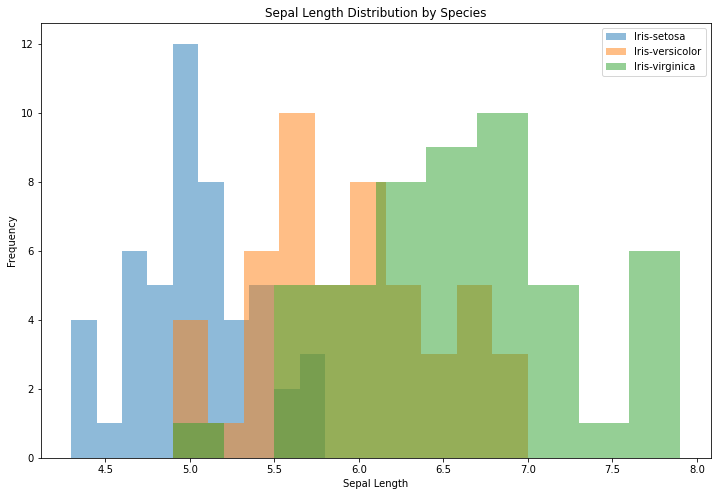
\includegraphics[width=80mm]{images/sepal_length.png}
  \caption{Histograma del largo del Sépalo}\label{fig1}
\end{figure}
\FloatBarrier

Como es posible apreciar en la primera figura, se creo un histograma sobre el largo de los sépalos para poder observar la distribución presentada entre las tres especies de flores. En este histograma se puede observar que los largos con mayor tendencia o frecuencia rondan sobre 5.0 , 5.5-6.0 y 6.5-7.0 para iris-setosa, iris-versicolor e iris-virginica respesctivamente.

\begin{figure}[ht]
  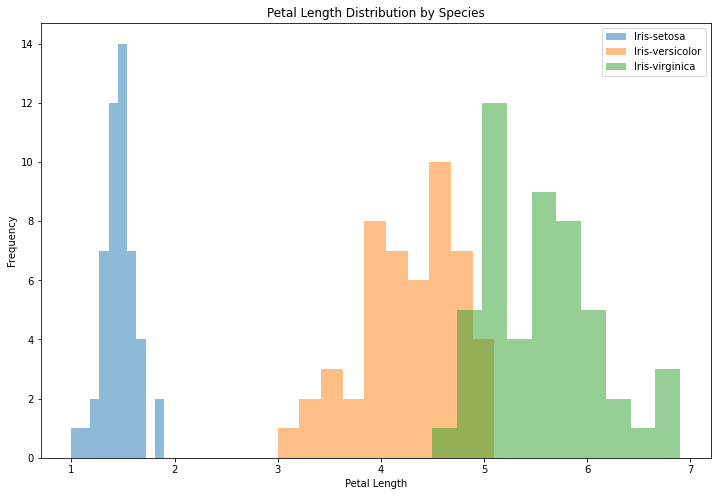
\includegraphics[width=80mm]{images/petal_length.png}
  \caption{Histograma del largo del Petalo}\label{fig2}
\end{figure}
\FloatBarrier

En el histograma del largo de los pétalos, se observa una distribución que varía significativamente entre las tres especies de flores. Para la especie Iris-setosa, la mayoría de los pétalos tienen una longitud concentrada en el rango de 1.0 a 2.0, mientras que para Iris-versicolor y Iris-virginica, la distribución se extiende a lo largo de un rango mayor, con los valores más comunes alrededor de 4.0 a 5.0 para Iris-versicolor y más cercana a 5.0 para Iris-virginica.

\begin{figure}[ht]
  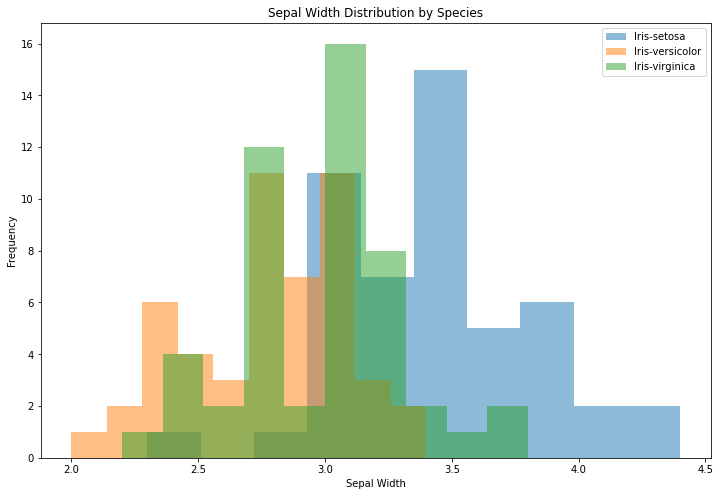
\includegraphics[width=80mm]{images/sepal_width.png}
  \caption{Histograma del ancho del Sepalo}\label{fig3}
\end{figure}
\FloatBarrier

El histograma del ancho de los sépalos muestra una distribución que difiere entre las especies de flores. Para Iris-setosa, la mayoría de los sépalos tienen un ancho concentrado principalmente en puntos cercanos a 3.5. Sin embargo, para Iris-versicolor y Iris-virginica, la distribución presentada tiene valores más comunes entre 2.5 y 3.5. La última distribución percibida es de 3.0 y 3.5 para Iris-virginica.

\begin{figure}[ht]
  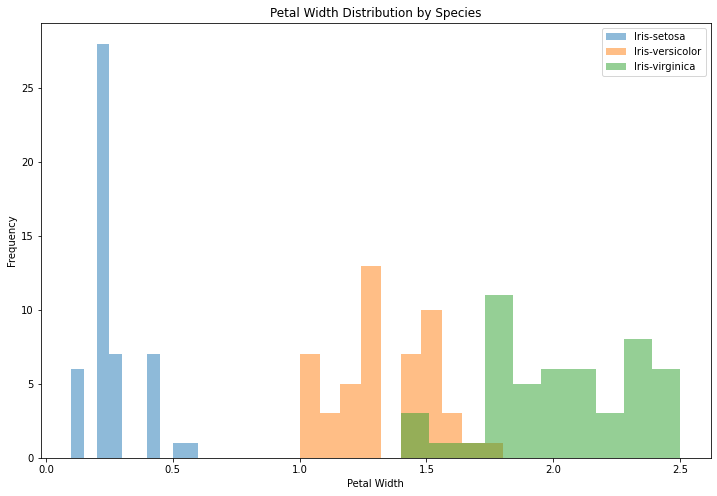
\includegraphics[width=80mm]{images/petal_width.png}
  \caption{Histograma del ancho del Petalo}\label{fig4}
\end{figure}
\FloatBarrier

En cuanto al ancho de los pétalos, se observa una clara diferencia entre las tres especies de flores. Para Iris-setosa, la mayoría de los pétalos tienen un ancho concentrado principalmente entre 0.0 y 0.5. Para Iris-versicolor, los valores más comunes se encuentran entre 1.0 y 1.5, mientras que para Iris-virginica, la distribución se extiende más ampliamente, con valores comunes entre 1.5 y 2.0.

\begin{figure}[ht]
  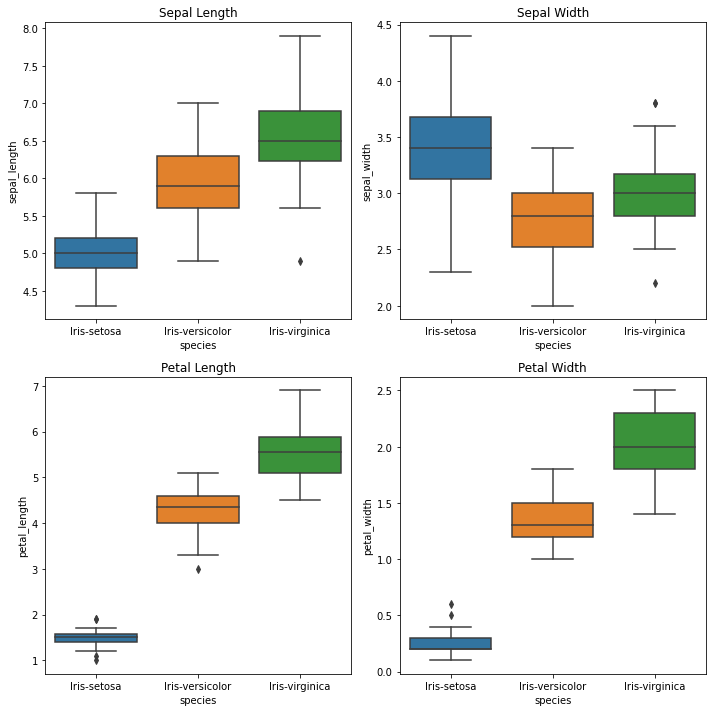
\includegraphics[width=80mm]{images/boxplot.png}
  \caption{Histograma del largo del Sépalo}\label{fig5}
\end{figure}
\FloatBarrier

El gráfico de boxplots mostrado ejemplifica que concentraciones promedio sobre las tendencias observadas en los histogramas anteriores están respaldadas por las concentraciones promedio de las características de las tres especies de flores. Los valores promedio de longitud y ancho de los sépalos y pétalos se alinean con las áreas de mayor frecuencia en los histogramas respectivos, lo que confirma la consistencia en la distribución de estas características entre las especies.

\section{Algoritmo de KNN}\label{AA}
El algoritmo de los k-Nearest Neighbors (KNN), según lo visto en clase, es un método simple y efectivo de aprendizaje supervisado utilizado para clasificación y regresión. La idea básica detrás de KNN es clasificar un punto de datos basándose en las clases de los puntos vecinos más cercanos.

\begin{figure}[ht]
  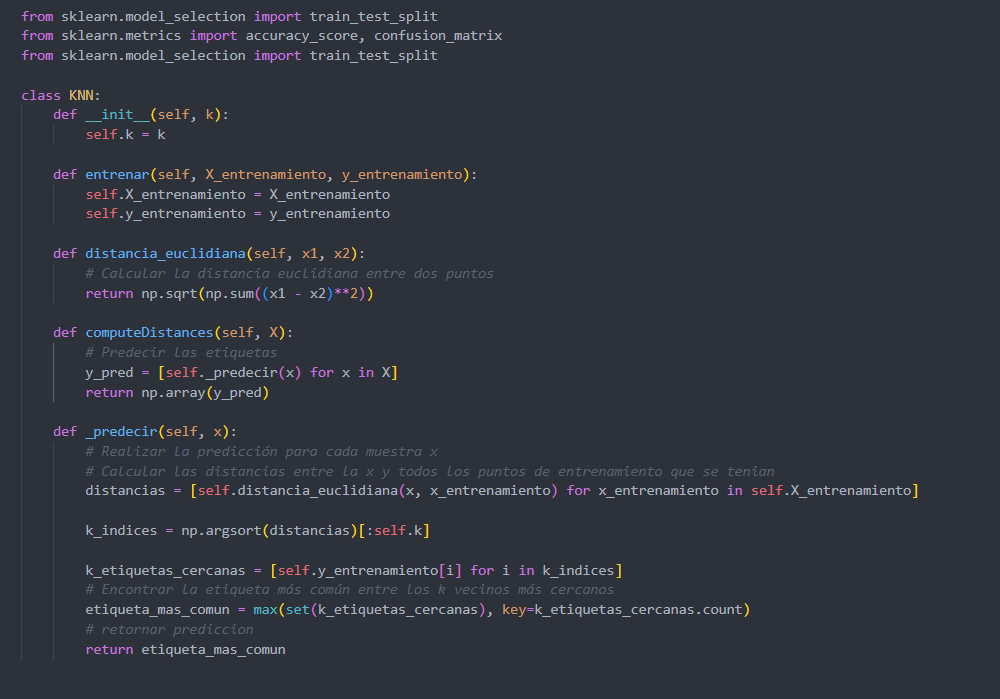
\includegraphics[width=80mm]{images/KNN.png}
  \caption{Algoritmo KNN}\label{fig6}
\end{figure}
\FloatBarrier

Esta versión del algoritmo es una ligera variación del algoritmo presentado en clase. En esta versión la fase de entrenamiento simplemente consta de memorizar los datos brindados del split de training. Por su parte la prediccion de clases de un punto x se realiza calculando las distancias entre el punto dado y los puntos de entrenamiento, una vez se calcula la distancia los puntos k que se selccionan y retornan son aquellos más cercanos a los datos de prueba.

\section{Resultados de Experimentacion}
En esta sección, se realizaron experimentos con diversos parámetros en el algoritmo KNN con el objetivo de mejorar su rendimiento en la clasificación de las especies de flores Iris. Se exploraron diferentes valores de k para determinar la combinación óptima de parámetros que maximizara la precisión del modelo.

Posteriormente, se evaluó el rendimiento del modelo KNN utilizando métricas de precisión. Estas métricas proporcionan una medida cuantitativa de la capacidad del modelo para clasificar correctamente las especies de flores Iris en el conjunto de datos de prueba. 

\begin{figure}[ht]
  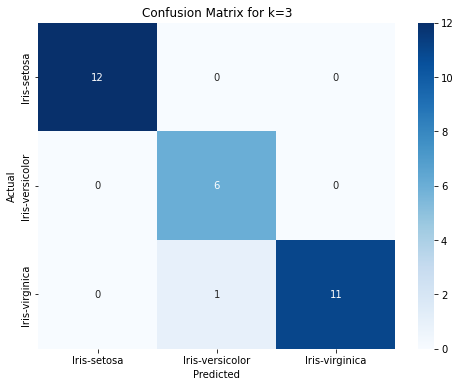
\includegraphics[width=80mm]{images/k3.png}
  \caption{K 3}\label{fig7}
\end{figure}
\FloatBarrier
En este primer experimento se decidió utilizar el número 3 como nuestro K. Esta exploración mostró en la matriz de confusión que; la primera y segunda clasificación se realizó de manera correcta, sin embargo, las predicciones de la tercera clase si presentó errores lo que arroja una precision de 0.9667. Esto nos indica que apesar de no ser perfecto tiene una precisión alta el modelo generado.
\begin{figure}[ht]
  \includegraphics[width=80mm]{images/K7.png}
  \caption{K 7}\label{fig8}
\end{figure}
\FloatBarrier
Este modelo tiene una precisión perfecta, lo que significa que todas las predicciones son correctas sobre el valor 7 escogido como K. La matriz de confusión confirma esto, mostrando que todas las muestras han sido clasificadas correctamente en sus respectivas clases.

\begin{figure}[H]
  \includegraphics[width=80mm]{images/K10.png}
  \caption{K 10}\label{fig9}
\end{figure}
\FloatBarrier

\begin{figure}[H]
  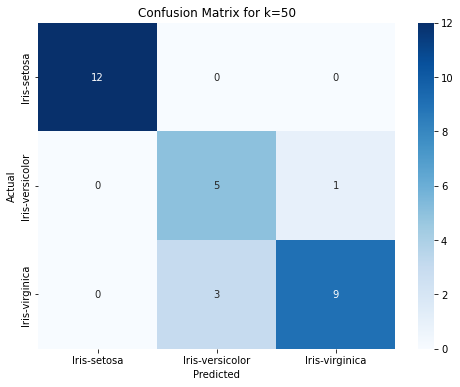
\includegraphics[width=80mm]{images/k50.png}
  \caption{K 50}\label{fig10}
\end{figure}
\FloatBarrier

Estas últimas dos matrices de confusión nos permiten notar que entre más grande resulta ser el número escogido sobre K y entre más se aleja de la predicción perfecta notada con 7, más baja la precisión y más aumentan los errores. Dando en los casos respectivos de 10 y 50 un 0.9667 y un 0.8667


\subsection{Conclusiones}
El proceso de elaboración de un modelo KNN (K-Nearest Neighbors) y la evaluación de características implican una serie de etapas cruciales para garantizar un rendimiento óptimo. Este proceso ayudo a la comprensión de diversos temas tratados a lo largo de las lecciones sobre las herramientas, algoritmos y modelos expuestos. Igualmente, fue una oportunidad de aprendizaje, por medio de la práctica real, sobre el funcionamiento de un modelo de Machine Learning para la evaluación de un conjunto de datos.


\begin{thebibliography}{00}
\bibitem{b1} Díaz, R. (2020, May 12). Algoritmo KNN - cómo funciona y ejemplos en Python. The Machine Learners. https://www.themachinelearners.com/algoritmo-knn/

\end{thebibliography}

\begin{figure}[ht]
  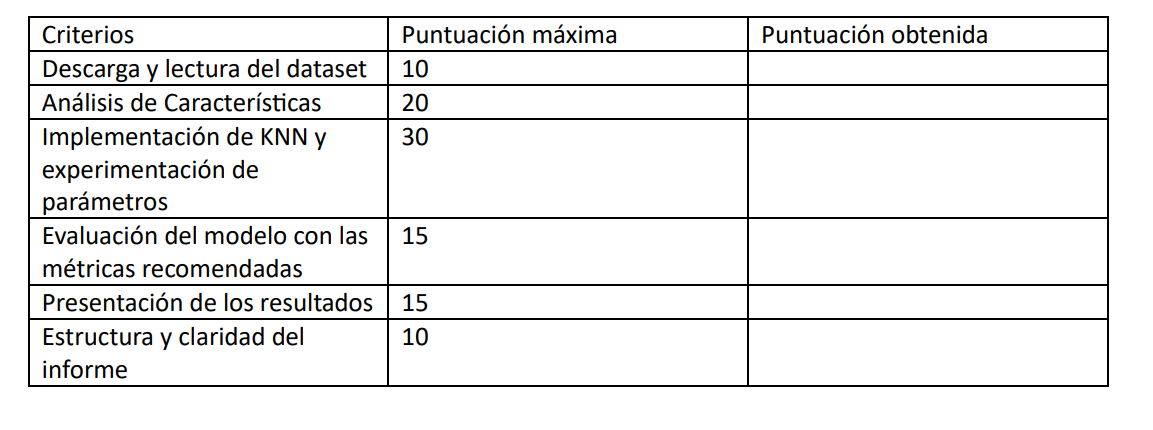
\includegraphics[width=80mm]{images/rubrica.png}
  \caption{Rubrica}\label{fig11}
\end{figure}
\FloatBarrier
\end{document}
